\documentclass[a4paper,french,bookmarks]{article}

\usepackage{./Structure/4PE18TEXTB}

\newboxans
\usepackage{booktabs}
\usepackage{tikz-3dplot}
 
\tdplotsetmaincoords{70}{122}

\begin{document}

    \renewcommand{\thesection}{\Roman{section}} 
    \renewcommand{\thesubsection}{\thesection.\Alph{subsection}}
    \setlist[enumerate]{font=\color{white5!60!black}\bfseries\sffamily}
    \renewcommand{\labelenumi}{\thesection.\arabic{enumi}.}
    \renewcommand*{\labelenumii}{\alph{enumii}.}
    \renewcommand*{\labelenumiii}{\alph{enumiii}.}
    
    \newcommand{\ON}{\mathbf{ON}}
    
    \stylizeDocSpe{Physique}{Devoir maison n° 12}{Théorème de Gauss et condensateurs}{Pour le mercredi 25 janvier 2023}
    
    \section{Théorème de Gauss}
    
    \begin{enumerate}
        \item Énoncer le théorème de \textsc{Gauss} relatif au flux sortant du champ électrostatique $\vec E$ à travers une surface fermée $\bcS$ contenant la charge électrique $Q_\text{int}$.
        
        \begin{theorem*}{Théorème de Gauss}{}
            \[ \hg{\boldsymbol\Phi\p{S} = \oiint_\bcS \vec E \cdot \dif \vec \bcS = \dfrac{Q_\text{int}}{\epsilon_0}}\]
                %
                où \hg{$\epsilon_0$} est la \hg{permittivité du vide}.
        \end{theorem*}
        
        \item Donner l'expression de l'équation de \textsc{Maxwell} qui permet de démontrer le théorème de \textsc{Gauss}.
        
        \noafter
        %
        \boxansconc{
            Le théorème de \textsc{Gauss} est une version intégrale de l'équation de \textsc{Maxwell-Gauss} :
            %
            \[ \mathrm{div} \vec E = \vec \nabla \cdot \vec E = \dfrac{\rho}{\epsilon_0}\]
            %
        }
        %
        \nobefore
        %
        \boxans{
            En effet, considérons un volume $\bcV$ de surface $\bcS$ (\ie $\partial \bcV = \bcS$) contenant une charge $Q_\text{int}$. On intègre
            %
            \[ \iiint_\bcV \vec \nabla \cdot \vec E \dif \tau_\bcV = \iiint_\bcV \dfrac{\rho}{\epsilon_0} \dif \tau_\bcV = \dfrac{Q_\text{int}}{\epsilon_0}\]
        }
        %
        \yesafter
        %
        \boxansconc{
            Or par \emph{théorème d'\textsc{Ostrogradski}}, $\displaystyle \iiint_\bcV \vec \nabla \cdot \vec E \dif \tau_\bcV = \oiint_{\bcS} \vec E \cdot \dif \vec \bcS$. On a bien montré le théorème de \textsc{Gauss}.
        }
        %
        \yesbefore
    \end{enumerate}
    
    \section{Condensateur plan}
    
    \begin{enumerate}
        \item En considérant les propriétés de symétrie de la distribution de charges, montrer que le champ électrostatique $\vec E$ créé par un plan infini uniformément chargé avec une densité surfacique $\sigma$ positive est orthogonal au plan. Démontrer que $\vec E$ est tel que sa norme vaut $E = \dfrac{\sigma}{2\epsilon_0}$. Représenter sur un schéma le vecteur $\vec E$ de part et d'autre du plan. On indiquera avec précision la surface de \textsc{Gauss} choisie.
        
        \noafter
        %
        \boxans{
            Considérons la base orthonormée directe $\p{O, \vec{e_x}, \vec{e_y}, \vec{e_z}}$ telle que $P\p{O, \vec{e_x}, \vec{e_y}}$ soit le plan en question. On a les plans de symétries $\Pi_\text S\p{M, \vec{e_x}, \vec{e_z}}$ et $\Pi_\text S'\p{M, \vec{e_y}, \vec{e_z}}$. On a alors $\vec E\p{M} \in \Pi_\text s \cap \Pi_\text s'$, d'où $\vec E\p{M} = E\p{M}\vec{e_z}$.
        }
        %
        \nobefore
        %
        \boxansconc{
            Le champ est donc bien orthogonal au plan.
        }
        %
        \boxans{
            \begin{minipage}{0.45\linewidth}
                \begin{center}
                    \tdplotsetmaincoords{70}{20}
                    \pgfplotsset{compat=newest}
                    
                    \begin{tikzpicture}[tdplot_main_coords, scale = 1.8]
                    
                        \draw[-latex,very thick,main10!70] (-1.3,0.7,0) --++ (0,0,-0.7)
                        node[midway,right] {$\vec E$};
                        
                        
                    
                        \fill[pattern=north west lines,opacity=0.5] (-1/2, -1/2, -1/2) -- (-1/2, 1/2, -1/2) -- (1/2, 1/2, -1/2) -- (1/2, -1/2, -1/2)  -- node[opacity=1,main3,below,midway] {$\quad\bcS\p{-z_0}$} cycle;
                        
                        \fill[main3!70,opacity=0.1] (-1/2, -1/2, -1/2) --   (-1/2, 1/2, -1/2) -- (-1/2, 1/2, 0) -- (-1/2, -1/2, 0) --cycle;
                        \fill[main3!70,opacity=0.1] (-1/2, 1/2, -1/2) -- (1/2, 1/2, -1/2) -- (1/2, 1/2, 0) -- (-1/2, 1/2, 0) -- cycle;
                    
                        \draw[main3!50!black] (-1/2, 1/2, 0) -- (-1/2, 1/2, -1/2);
                    
                        \fill[main3!70,opacity=0.5] (-1/2, -1/2, -1/2) -- (1/2, -1/2, -1/2) -- (1/2, -1/2, 0) -- (-1/2, -1/2, 0) -- cycle;
                    
                        \draw[main3!50!black,fill=main3!70,opacity=0.5] (-1/2, -1/2, -1/2) -- (-1/2, 1/2, -1/2) -- (1/2, 1/2, -1/2) -- (1/2, -1/2, -1/2) -- cycle;
                        
                        \fill[main3!70,opacity=0.5] (1/2, -1/2, 0) -- (1/2, 1/2, 0) -- (1/2, 1/2, -1/2) -- (1/2, -1/2, -1/2) -- cycle;
                        
                        \draw[main3!50!black] (-1/2, -1/2, 0) -- (-1/2, -1/2, -1/2);
                        \draw[main3!50!black] (1/2, -1/2, 0) -- (1/2, -1/2, -1/2);
                        \draw[main3!50!black] (1/2, 1/2, 0) -- (1/2, 1/2, -1/2);
    
                        \draw[dashed, gray] (0,0,0) -- (0,0,-0.5);
                        \draw[dashed, gray] (0,0,0) -- (0,-1.5, 0);
                        \draw[dashed, gray] (0,0,0) -- (-1.5, 0, 0);
                        
                        \draw[-latex,very thick,main10!70] (1.2,1,0) --++ (0,0,-0.7);
                        
                        \draw[-latex,very thick,main10!70] (0.7,-0.5,0) --++ (0,0,-0.7);
                    
                        \draw[dashed,main3,fill=main3!30,opacity=0.5] (-1.5, -1.5, 0) -- (-1.5, 1.5, 0) -- (1.5, 1.5, 0) -- (1.5, -1.5, 0) node[main3, above] {$P$} -- cycle;
                        
                        \draw[main3!50!black] (-1/2, 1/2, 0) -- (-1/2, 1/2, 1/2);
                        
                        \draw[-stealth] (0,0,0) node[above left] {$O$} -- (0,0,1)
                            node[above] {$z$};
                            
                        \draw[-stealth] (0,0,0)-- (1.8,0,0)
                            node[above] {$x$};
                            
                        \draw[-stealth] (0,0,0)-- (0,1.8,0)
                            node[above] {$y$};
                            
                        \fill[pattern=north west lines,opacity=0.1] (-1/2, -1/2, 0) -- (-1/2, 1/2, 0) -- (1/2, 1/2, 0) -- (1/2, -1/2, 0)  -- cycle;
                            
                        \draw[white] (-1/2, -1/2, 0) -- (-1/2, 1/2, 0) -- (1/2, 1/2, 0) -- (1/2, -1/2, 0) -- cycle;
                        
                        \fill[main3!70,opacity=0.1] (-1/2, -1/2, 1/2) -- (-1/2, 1/2, 1/2) -- (-1/2, 1/2, 0) -- (-1/2, -1/2, 0) -- cycle;
                        \fill[main3!70,opacity=0.1] (-1/2, 1/2, 1/2) -- (1/2, 1/2, 1/2) -- (1/2, 1/2, 0) -- (-1/2, 1/2, 0) -- cycle;
                        
                        \fill[main3!70,opacity=0.5] (1/2, -1/2, 0) -- (1/2, 1/2, 0) -- (1/2, 1/2, 1/2) -- (1/2, -1/2, 1/2) -- cycle;
                        
                        \fill[pattern=north west lines,opacity=0.5] (-1/2, -1/2, 1/2) -- (-1/2, 1/2, 1/2) -- (1/2, 1/2, 1/2) -- (1/2, -1/2, 1/2)  -- cycle;
                        
                        \draw[main3!50!black,fill=main3!70,opacity=0.5] (-1/2, -1/2, 1/2) -- (-1/2, 1/2, 1/2) -- node[opacity=1,main3,above,midway] {$\quad\bcS\p{z_0}$} (1/2, 1/2, 1/2) -- (1/2, -1/2, 1/2)  -- cycle;
                        
                        \draw[-latex,very thick,main10!70] (-1.3,0.7,0) --++ (0,0,0.7)
                        node[midway,right] {$\vec E$};
                        \draw[-latex,very thick,main10!70] (1.2,1,0) --++ (0,0,0.7);
                        
                        \draw[-latex,very thick,main10!70] (0.7,-0.5,0) --++ (0,0,0.7);
                        
                        
                        \fill[main3!70,opacity=0.5] (-1/2, -1/2, 1/2) -- (1/2, -1/2, 1/2) -- (1/2, -1/2, 0) -- (-1/2, -1/2, 0) -- cycle;
                        
                        \draw[main3!50!black] (-1/2, -1/2, 0) -- (-1/2, -1/2, 1/2);
                        \draw[main3!50!black] (1/2, -1/2, 0) -- (1/2, -1/2, 1/2);
                        \draw[main3!50!black] (1/2, 1/2, 0) -- (1/2, 1/2, 1/2);
                    \end{tikzpicture}
                \end{center}
            \end{minipage}
            %
            \begin{minipage}{0.55\linewidth}
                La distribution de charge étant invariante par translation selon $\vec{e_x}$ et $\vec{e_y}$, on a $\vec E\p{x, y, z} = E\p{z}\vec{e_z}$. Considérons le volume $\bcV$ correspondant à un pavé centré en $O$, de hauteur $2z_0 \geq 0$, de profondeur égale à $1$, et de largeur égale à $1$. Notons $\bcS$ la surface correspondant à un carré de côté $1$ centré en $O$, autrement dit l'intersection du volume avec le plan, de vecteur normal $1^2\times\vec{e_z} = \vec{e_z}$. Les faces latérales étant de vecteur normal selon $\vec{e_x}$ ou $\vec{e_y}$, le flux sortant à travers ces faces est nul. Le flux sortant à travers la surface du cube est donc donné par des copies $\bcS\p{z_0}$ et $\bcS\p{-z_0}$ de $\bcS$ en $z = z_0$ et $z = -z_0$. 
            \end{minipage}
            %
            \[ \oiint_{\partial \bcV} E\p{z}\vec{e_z} \cdot \dif \vec{\bcS} = \oiint_{\bcS\p{z_0}} E\p{z_0}\vec{e_z} \cdot \vec{e_z} + \oiint_{\bcS\p{-z_0}} E\p{-z_0}\vec{e_z} \cdot \p{-\vec{e_z}} + 0 = E\p{z_0} - E\p{-z_0}\]
            %
            Le plan $P$ étant un plan de symétrie, on a $E\p{-z_0} = -E\p{z_0}$ et $E\p{z_0} - E\p{-z_0} = 2E\p{z_0}$. La charge électrique $Q_\text{int}$ contenue dans $\bcV$ est donnée par l'intersection de $\bcV$ et $P$, autrement dit par $\bcS$, d'où $Q_\text{int} = \sigma$. 
        }
        \yesafter
        %
        \boxansconc{
            Le \emph{théorème de \textsc{Gauss}} livre enfin $2E\p{z_0} = \dfrac{Q_\text{int}}{\epsilon_0} = \dfrac{\sigma}{\epsilon_0}$, donc finalement $E\p{z_0} = E = \dfrac{\sigma}{2\epsilon_0}$.
        }
        %
        \yesbefore
    \end{enumerate}
    
    \begin{minipage}{0.5\linewidth}
        Soit un condensateur plan constitué par deux plans infinis, parallèles, uniformément chargés et séparés par une distance $d$. La plan supérieur étant chargé avec une densité surfacique $\sigma$ positive et le plan inférieur étant chargé avec une densité $-\sigma$.
    \end{minipage}
    %
    \begin{minipage}{0.5\linewidth}
        \begin{center}
            \begin{tikzpicture}[cross/.style={path picture={
                \draw[black] (path picture bounding box.south east) -- (path picture bounding box.north west) (path picture bounding box.south west) -- (path picture bounding box.north east);
            }}]
                \draw[<->] (0.15, -0.8) --++ (0, 1.6) node[midway, left] {$d$};
                    
                \draw[thick, main3] (0.4, 0.8) --node[pos=0.8, above]  {$+\sigma$} ++ (5, 0);
                \draw[thick, main3] (0.4, -0.8) --node[pos=0.8, below] {$-\sigma$} ++ (5, 0);
                    
                \draw[->] (6.7, 0.3) --++ (0.7, 0) node[right] {$\vec{e_x}$};
                \draw[->] (6.7, 0.3) --++ (0, 0.7) node[right] {$\vec{e_z}$};
                \node[draw,circle,cross,minimum width=0.3cm] at (6.7, 0.3){};
                    
                \node[fill=main3,circle,inner sep=1pt,label={[font=\footnotesize,main3]north east:$O$}] at (2.9, 0){};
                    
                \node at (6.7, -0.15) {$\vec{e_y}$}; 
            \end{tikzpicture}
        \end{center}
    \end{minipage}
    %
    \begin{enumerate}[resume]
        \item En utilisant le théorème de superposition, déduire de la question précédente le champ en tout point de l'espace.
        \noafter
        %
        \boxans{
            Notons $\vec{E_+}$ et $\vec{E_-}$ les champs électrostatiques créés respectivement par le plan supérieur et inférieur, et posons $E = \dfrac{\sigma}{2\epsilon_0}$. Pour un point $M\p{x, y, z}$ on a 
            %
            \[ \vec{E_+}\p{M} = \left\lbrace\begin{array}{cl}
                E\vec{e_z} &\text{si} \ z \geq \sfrac{d}{2}  \\
                -E\vec{e_z} &\text{sinon}
            \end{array}\right. \qquad\et\qquad \vec{E_-}\p{M} = \left\lbrace\begin{array}{cl}
                -E\vec{e_z} &\text{si} \ z \geq -\sfrac{d}{2}  \\
                E\vec{e_z} &\text{sinon}
            \end{array}\right.\]
            %
        }
        \nobefore\yesafter
        %
        \boxansconc{
            Par \emph{théorème de superposition}, le champ électrique au point $M\p{x, y, z}$ vaut
            %
            \begin{enumerate}
                \itt $\vec 0$ si le point $M$ est au-dessus du plan supérieur, car $\vec{E_+}\p{M} + \vec{E_-}\p{M}= \p{E - E}\vec{e_z}$.
                
                \itt $\vec 0$ si le point $M$ est en-dessous du plan inférieur, car $\vec{E_+}\p{M} + \vec{E_-}\p{M}= \p{-E + E}\vec{e_z}$.
                
                \itt $\dfrac{\sigma}{\epsilon_0}\vec{e_z}$ si le point $M$ est entre les deux plans, car $\vec{E_+}\p{M} + \vec{E_-}\p{M}= -2E\vec{e_z} = -\dfrac{\sigma}{\epsilon_0}\vec{e_z}$.
            \end{enumerate}
        }
        %
        \yesbefore
        
        \item Déterminer la différence de potentiel $U$ entre les deux plans du condensateur. On exprimera $U$ en fonction de $\epsilon_0$, $\sigma$ et $d$.
        
        \boxansconc{
            On considère le point $A\p{0, 0, -\sfrac{d}{2}}$ du plan inférieur et le point $B\p{0, 0, \sfrac{d}{2}}$ du plan supérieur. On a directement 
            %
            \[ U = \mod{V\p{B} - V\p{A}} = \mod{\int_A^B \vec{E}\cdot \dif \vec \ell} = \int_{-\sfrac{d}{2}}^{\sfrac{d}{2}} E\p{z}\dif z = \dfrac{\sigma}{\epsilon_0}\int_{-\sfrac{d}{2}}^{\sfrac{d}{2}} \dif z = \dfrac{\sigma d}{\epsilon_0}\]
        }
        
        \item Définir et déterminer la capacité $C$ du condensateur par unité de surface. Exprimer $C$ en fonction de $\epsilon_0$ et $d$.
        
        \noafter
        %
        \boxans{
            Pour une surface finie $\bcS$ contenant la charge $Q$, la capacité d'un condensateur est généralement définie comme la quantité $C_\bcS$ telle que $U = \dfrac{Q}{C_\bcS}$. La capacité par unité de surface est alors $C = \dfrac{C_\bcS}{\bcS} = \dfrac{Q\epsilon_0}{\bcS\sigma d}$. Or pour une densité surface uniforme $\sigma$ de charge, on a $Q = \bcS\sigma $, d'où $C = \dfrac{\bcS\sigma \epsilon_0}{\bcS\sigma  d} = \dfrac{\epsilon_0}{d}$. On peut conserver cette définition 
        }
        %
        \nobefore\yesafter
        %
        \boxansconc{
            dans le cas d'un plan infini :
            %
            \[ C = \dfrac{\epsilon_0}{d}\]
        }
        %
        \yesbefore
    \end{enumerate}
        
    \begin{minipage}{0.5\linewidth}
        On introduit entre les deux plaques du condensateur plan précédent une plaque métallique parallélépipédique d'épaisseur $e < d$ parallèle aux armatures du condensateur. L'épaisseur $e$ est donc une grandeur finie, mais on considère infinies les autres dimensions de la plaque.
    \end{minipage}
    %
    \begin{minipage}{0.5\linewidth}
        \begin{center}
            \begin{tikzpicture}[cross/.style={path picture={
                \draw[black] (path picture bounding box.south east) -- (path picture bounding box.north west) (path picture bounding box.south west) -- (path picture bounding box.north east);
            }}]
                \draw[<->] (0.15, -0.3) --++ (0, 0.6) node[midway, left] {$e$};
                    
                \draw[thick, main3] (0.4, 0.8) --node[pos=0.7,above] {$+\sigma$} ++ (5, 0) node[right] {$\p{\Pi}$};
                \draw[thick, main3] (0.4, -0.8) --node[pos=0.7,below] {$-\sigma$}++ (5, 0) node[right] {$\p{\Pi'}$};
                    
                \draw[->] (6.7, 0.3) --++ (0.7, 0) node[right] {$\vec{e_x}$};
                \draw[->] (6.7, 0.3) --++ (0, 0.7) node[right] {$\vec{e_z}$};
                \node[draw,circle,cross,minimum width=0.3cm] at (6.7, 0.3){};
                    
                \node at (6.7, -0.15) {$\vec{e_y}$}; 
                    
                \fill[main3!15] (0.4, 0.3) rectangle (5.4, -0.3);
                \draw[thick, main3] (0.4, 0.3) --++ (5, 0) node[right] {$\p{P}$};
                \draw[thick, main3] (0.4, -0.3) --++ (5, 0) node[right] {$\p{P'}$};
            \end{tikzpicture}
        \end{center}
    \end{minipage}
    %
    \begin{enumerate}[resume]
        \item On admet que le champ électrostatique est nul à l'intérieur du métal. Justifier le fait qu'il apparaîtra des charges électriques sur les surfaces supérieure $\p{P}$ et $\p{P'}$ de la plaque métallique, et déterminer le signe de ces charges.
        
        \noafter
        %
        \boxans{
            Soient $\vec{E_1}$ le champ créé par les deux plaques du condensateur, et $\vec{E_2}$ celui créé par la plaque métallique. Soit $M$ un point situé à l'intérieur de la plaque métallique, par \emph{théorème de superposition}, on a 
            %
            \[ \vec{E_1}\p{M} + \vec{E_2}\p{M} = \vec{0} \qquad\text{donc}\qquad \vec{E_1}\p{M} = -\vec{E_2}\p{M}\]
            %
            La plaque métallique génère donc un champ électrostatique s'opposant à celui du condensateur. Pour ce faire, il faut que les porteurs de charges la constituant (électrons, \dots) se déplacent sur les extrémités du métal. Le champ se dirige des charges positives vers les négatives, donc $\vec{E_1}$ va de $\p{\Pi}$ vers $\p{\Pi'}$. Ainsi $\vec{E_2} = -\vec{E_1}$ va dans l'autre sens, \ie de $\p{P'}$ vers $\p{P}$. Donc :
        }
        %
        \nobefore\yesafter
        %
        \boxansconc{
            \begin{enumerate}
                \itt Les charges qui apparaissent sur la surface supérieure $\p{P}$ sont chargées négativement.
                
                \itt Les charges qui apparaissent sur la surface inférieure $\p{P'}$ sont chargées positivement.
            \end{enumerate}
        }
        %
        \yesbefore
        
        \item En utilisant le théorème de \textsc{Gauss} sur une surface que l'on précisera, déterminer et exprimer en fonction de $\sigma$ les densités surfaciques de charge $\sigma_P$ et $\sigma_{P'}$ qui apparaissent sur les surfaces $\p{P}$ et $\p{P'}$ de la plaque métallique.
        
        \noafter
        %
        \boxans{
            Considérons $\bcS$ une carré de côté $1$ situé en $M\p{0, 0, \dfrac{d + e}{2}}$ de vecteur normal $\vec{e_z}$. On extrude symétriquement ce carré selon $\vec{e_z}$ pour obtenir un pavé $\bcV$ de hauteur $\dfrac{d - e}{2} + \dif z$. Le champ étant porté par $\vec{u_z}$, le flux sortant des faces latérales est nul. Par ailleurs, la face supérieure est située $\dif z$ au dessus de $\p{\Pi}$ et celle inférieure $\dif z$ en dessous de $\p{P}$, où le champ est nul :
            %
            \[ \oiint_{\partial \bcV} \vec E\p{z}\cdot \dif \vec{\bcS} = \oiint_{\bcS\p{\sfrac{e}{2} - \dif z}} E\p{\dfrac{e}{2} - \dif z} + \oiint_{\bcS\p{\sfrac{d}{2} + \dif z}} E\p{\dfrac{d}{2} + \dif z} = 0\]
            %
            Par le même principe, la charge intérieure à $\bcV$ est $Q_\text{int} = \sigma + \sigma_P$. Par \emph{théorème de \textsc{Gauss}}, on obtient donc
            %
        }
        \nobefore\yesafter
        %
        \boxansconc{
            \[ \dfrac{\sigma + \sigma_P}{\epsilon_0} = 0 \qquad\text{donc}\qquad \sigma_P = -\sigma\]
            %
            Le même principe s'applique symétriquement pour obtenir $\sigma_{P'} = -\p{-\sigma}$, d'où $\sigma_{P'} = \sigma = -\sigma_{P}$.
        }
        %
        \yesbefore
        
        \item Déterminer la valeur du champ électrostatique en un point du condensateur extérieur à la plaque métallique (entre $P$ et $\Pi$ d'une part et entre $P'$ et $\Pi'$ d'autre part).
        
        \boxansconc{
            Un point $M$ situé entre $\p{\Pi}$ et $\p{P}$ est comme situé entre une plaque supérieure infinie chargée selon $\sigma$, et une plaque inférieure infinie chargée selon $-\sigma$. La situation est donc similaire aux questions précédentes, et on a
            %
            \[ \vec E\p{M} = -\dfrac{\sigma}{\epsilon_0}\vec{e_z} = 2E\]
            
            Symétriquement pour $M'$ entre $\p{P'}$ et $\p{\Pi'}$, on a $\vec E\p{M'} = \dfrac{\sigma}{\epsilon_0}\vec{e_z} = -2E$.
        }
        
        \item En déduire la capacité surfacique $C'$ du condensateur ainsi obtenu. On exprimera $C'$ en fonction de $e$, $d$ et $\epsilon_0$. Conclure quant à l'influence de la plaque métallique sur la capacité surfacique du condensateur.
        
        \noafter
        %
        \boxans{
            On considère les mêmes points $A$ et $B$, et on a cette fois
            %
            \begin{align*}
                U &= \mod{V\p{B} - V\p{A}} = \int_{-\sfrac{d}{2}}^{-\sfrac{e}{2}} E\p{z}\dif z + \int_{\sfrac{e}{2}}^{\sfrac{d}{2}} E\p{z}\dif z\\ 
                &= 2E\p{\dfrac{-e}{2} - \dfrac{-d}{2} + \dfrac{d}{2} - \dfrac{e}{2}} = 2E\p{d - e} = \dfrac{\sigma\p{d - e}}{\epsilon_0}
            \end{align*}
        }
        %
        \nobefore\yesafter
        %
        \boxansconc{
            Par la même méthode, on obtient $C = \dfrac{\epsilon_0}{\p{d - e}}$. La plaque augmente donc la capacité surfacique du condensateur, agissant comme si elle avait rapproché les plaques. 
        }
    \end{enumerate}
    
    \section{Condensateur cylindrique}
    
    \begin{minipage}{0.5\linewidth}
        \resizebox{\linewidth}{!}{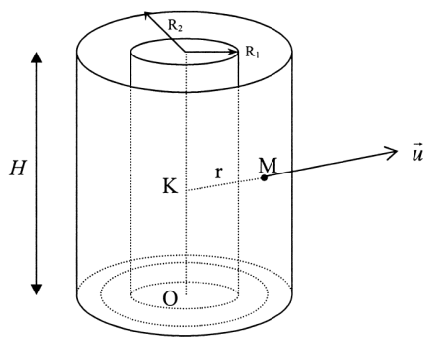
\includegraphics[]{dm12fig/dm12fig1.png}}
    \end{minipage}
    %
    \begin{minipage}{0.5\linewidth}
        On considère un condensateur cylindrique composé de deux armatures coaxiales de hauteur $H$ et de rayons respectifs $R_1$ et $R_2$ avec $R_1 < R_2$ et placées dans l'air. L'armature interne porte la charge électrique $Q > 0$. L'armature externe porte une charge totale $-Q$. Les potentiels électriques des armatures sont respectivement $V_1$ et $V_2$. Soit un point $M$ situé à la distance $r = KM$  de l'axe $R_1 < r < R_2$. $K$ est la projection orthogonale du point $M$ sur l'axe du condensateur.\medskip
        
        Soit $\vec u$ le vecteur unitaire de la droite $\p{KM}$ dirigé de $K$ vers $M$. On admettra que le champ électrostatique $\vec E$ créé au point $M$ est radial et sa norme ne dépend que de $r$, et on écrira donc $\vec E = E\p{r}\vec u$. On négligera les effets de bord.
    \end{minipage}
    
    
    
    \begin{enumerate}
        \item En appliquant le théorème de \textsc{Gauss} à une surface $\bcS$ que l'on précisera, déterminer l'expression de $E\p{r}$ en fonction de $Q$, $\epsilon_0$, $r$ et $H$. On distinguera les cas selon $r < R_1$, $R_1 \leq r < R_2$ ou $R_2 \leq r$.
        
        \noafter
        %
        \boxans{
            Supposons qu'il existe un unique cylindre de rayon $R$ et de hauteur $H$ selon $\vec{e_z} = \dfrac{\vec{OK}}{OK}$ portant la charge $Q$.
            
            On considère $\bcV$ un cylindre cylindre identique mais de rayon $r$. Par \emph{théorème de \textsc{Gauss}}
            %
            \[ \oiint_{\partial V} \vec E\p{M}\cdot \dif \vec{S} = 2\pi rHe\p{r} = \dfrac{Q_\text{int}}{\epsilon_0} \qquad\text{donc}\qquad E\p{r} = \begin{cases}\dfrac{Q}{2\pi\epsilon_0rH} &\text{si} \ r \geq R\\0 &\text{sinon}\end{cases}  \]
            %
            Par \emph{théorème de superposition} avec les deux cylindre de l'énoncé, on obtient 
        }
        %
        \nobefore\yesafter
        %
        \boxansconc{
            \[ E\p{r} = \begin{cases}\dfrac{Q}{2\pi \epsilon_0 rH} & \text{si} \ r \in \intor{R_1, R_2}\\
            0 &\text{sinon}\end{cases}\]
        }
        %
        \yesbefore
        
        \item En déduire le potentiel $V\p{r}$ à une distance $r$ de l'axe lorsque $R_1 < r < R_2$. On exprimera $V\p{r}$ en fonction de $Q$, $H$, $V_1$, $R_1$, $\epsilon_0$ et $r$. En déduire la différence de potentiel $U = V_1 - V_2$ entre les deux armatures en fonction de $Q$, $\epsilon_0$, $H$, $R_1$ et $R_2$.
        
        \noafter
        %
        \boxans{
            Comme dans les parties précédentes, on a 
            %
            \[ V\p{r} - V_1 = \int_{R_1}^r E\p{\ell}\dif \ell = \dfrac{Q}{2\pi \epsilon_0 H}\int_{R_1}^r \dfrac{\dif \ell}{\ell} = \dfrac{Q}{2\pi \epsilon_0 H}\ln{\dfrac{r}{R_1}} \]
        }
        %
        \nobefore\yesafter
        %
        \boxansconc{
            On a donc $V\p{r} = V_1 + \dfrac{Q}{2\pi \epsilon_0 H}\ln{\dfrac{r}{R_1}}$. Ainsi
            %
            \[ U = V_1 - V_2 = V_1 - V\p{R_2} = \dfrac{Q}{2\pi \epsilon_0 H}\ln{\dfrac{R_2}{R_1}}\]
        }
        %
        \yesbefore
        
        \item Déterminer la capacité $C$ du condensateur en fonction de $\epsilon_0$, $H$, $R_1$ et $R_2$.
        
        \boxansconc{
            On a par définition $U = \dfrac{Q}{C}$, d'où $C = \dfrac{2\pi \epsilon_0 H}{\ln{R_2} - \ln{R_1}}$
        }
        
        \item On peut associer au champ électrostatique une densité volumique d'énergie $\bcw_\text{el}$ égale à $\sfrac{1}{2}\epsilon_0 E^2$. En utilisant l'expression de $E\p{r}$ déterminée précédemment déterminée et en intégrant l'expression de $\bcw_\text{el}$, déterminer l'énergie $\bcW_\text{cond}$ accumulée par le condensateur en fonction de $Q$, $\epsilon_0$, $H$, $R_1$ et $R_2$, puis en fonction de $Q$ et $C$.
        
        \boxansconc{
            \[ \bcW_\text{cond} = \iiint \bcw_\text{el} = \dfrac{1}{2}\epsilon_0\int_{R_1}^{R_2} 2\pi r H E\p{r}^2\dif r = \dfrac{Q^2}{4\pi H}\int_{R_1}^{R_2} \dfrac{\dif r}{r} = \dfrac{Q^2}{4\pi \epsilon_0 H}\ln{\dfrac{R_2}{R_1}} = \dfrac{Q^2}{C}\]
        }
        
        \item En effectuant un développement limité de l'expression de la capacité déterminée à la question $9$, montrer que si les rayons des armatures sont très proches, c'est-à-dire si $R_2 - R_1 = e \ll R_1$, le condensateur cylindrique est à équivalent à un condensateur plan dont on précisera les caractéristiques.
        
        
        
        \noafter
        %
        \boxans{
            On a
            %
            \[ C = \dfrac{2\pi \epsilon_0 H}{\ln{\dfrac{R_2}{R_1}}} = \dfrac{2\pi \epsilon_0 H}{\ln{1 + \dfrac{e}{R_1}}} \approx \dfrac{2\pi\epsilon_0 HR_1}{e} = \p{2\pi R_1 H}\dfrac{\epsilon_0}{e}\]
            %
            La surface du premier cylindre étant $2\pi R_1 H$, la capacité par unité de surface est $C' = \dfrac{\epsilon_0}{e}$.
        }
        %
        \nobefore\yesafter
        %
        \boxansconc{
            Le condensateur cylindrique est donc équivalent à un condensateur créé par deux plaques infinies séparées par la distance $e = R_2 - R_1$.
        }
        %
        \yesbefore
    \end{enumerate}
    
    
\end{document}